% Results — Paper 2, Medical Physics submission
% Humanised v1, 2026-05-25. Formal-academic-active register, citation-bound.
% Numerical values verified 2026-05-25 against results/icc_table.csv,
% results/downstream_metrics.csv, and results/downstream_metrics_by_stratum.csv.

\subsection{Cohort}

The inclusion cascade screened 1\,018 LIDC-IDRI patient series~\cite{armato2011} via the pylidc-clustered annotation interface~\cite{hancock2016pylidc}; 600 patient series were downloaded from TCIA~\cite{clark2013} across two batches, and 353 annotated nodules met the pre-specified inclusion criteria (\S\,2.2). The primary analysis cohort, after seeded balanced downsampling of the malignant class, comprised 310 nodules (155 malignant, 155 benign) drawn from 227 unique patients (Table~1). Benign nodules clustered toward the lower diameter range (median 7.74~mm, IQR 6.70--9.20~mm), and malignant nodules spanned a wider distribution toward larger sizes (median 19.36~mm, IQR 14.30--25.58~mm). This size-class asymmetry is a structural property of LIDC-IDRI and is addressed quantitatively in \S\,3.5. Of the 310 cohort nodules, 65\% carried segmentations from all four LIDC readers and 35\% from three. The median pairwise inter-reader Dice similarity coefficient was 0.789 (mean 0.769, range 0.156--0.934), consistent with previously published LIDC inter-reader values of 0.75--0.80~\cite{kalpathycramer2016}, supporting the external validity of the perturbation-magnitude calibration. The per-nodule perturbation-condition count $K$ ranged from 7 to 12 across the 353-nodule extraction superset, reflecting the volume-preservation guard's intentional skipping of erosions that would have retained less than 25\% of the consensus-mask voxel count. The retention rate was 48\% for E1, 13\% for E2, and 2\% for E3; all dilation, translation, and Dice-calibrated perturbations were retained for every nodule.

\subsection{Per-feature stability under segmentation perturbation (H1)}

Across the ten universal perturbation conditions, both handcrafted radiomics and BiomedCLIP embeddings achieved high proportions of features classified as stable (ICC(2,1) $\geq 0.75$): 91.2\% for PyRadiomics-2D (93 of 102 features), 94.4\% for PyRadiomics-3D (101 of 107), and 90.4\% for BiomedCLIP (463 of 512 dimensions). Pre-registered two-proportion z-tests of the BiomedCLIP-versus-radiomics contrasts yielded no statistically significant difference at Bonferroni-corrected $\alpha = 0.025$: BiomedCLIP versus PyRadiomics-2D, $\Delta = -0.8$ percentage points, $z = -0.25$, $p = 0.80$; BiomedCLIP versus PyRadiomics-3D, $\Delta = -4.0$~pp, $z = -1.32$, $p = 0.19$. \textbf{Hypothesis H1 is rejected:} pretrained foundation-model embeddings are not, on aggregate, more stable than IBSI-aligned handcrafted radiomic features under segmentation-mask perturbation.

\subsection{Distribution-shape divergence (H1$'$)}

The aggregate-proportion analysis in \S\,3.2 conceals a qualitative divergence between paradigms that is visible in the ICC stratum crosstab (Figure~2a) and the empirical cumulative distribution functions (Figure~2b). PyRadiomics exhibits a bimodal stability profile: 62.6\% of 3D features and 67.6\% of 2D features fall in the excellent stratum (ICC $\geq 0.90$), with the remainder distributed across moderate, good, and a small unstable tail (one feature in each radiomics arm with ICC $<$ 0.50). BiomedCLIP exhibits a unimodal moderate-stability profile: only 1 of 512 dimensions reaches the excellent stratum, 90.2\% concentrate in the good stratum ($0.75 \leq$ ICC $<$ 0.90), and zero dimensions fall in the poor stratum. The pre-specified two-sample Kolmogorov--Smirnov tests confirm that the two paradigms behave as categorically distinct populations of features: BiomedCLIP versus PyRadiomics-2D, $D = 0.722$, $p = 3.2 \times 10^{-44}$; BiomedCLIP versus PyRadiomics-3D, $D = 0.679$, $p = 4.3 \times 10^{-40}$. A secondary comparison between the two PyRadiomics arms yields a small but statistically significant difference ($D = 0.246$, $p = 0.003$), with the 2D arm sitting marginally closer to the excellent stratum than the 3D arm. \textbf{Hypothesis H1$'$ (distribution-shape divergence between paradigms) is strongly supported} and is reported as the primary novel finding of this study.

\begin{figure}[H]
\centering
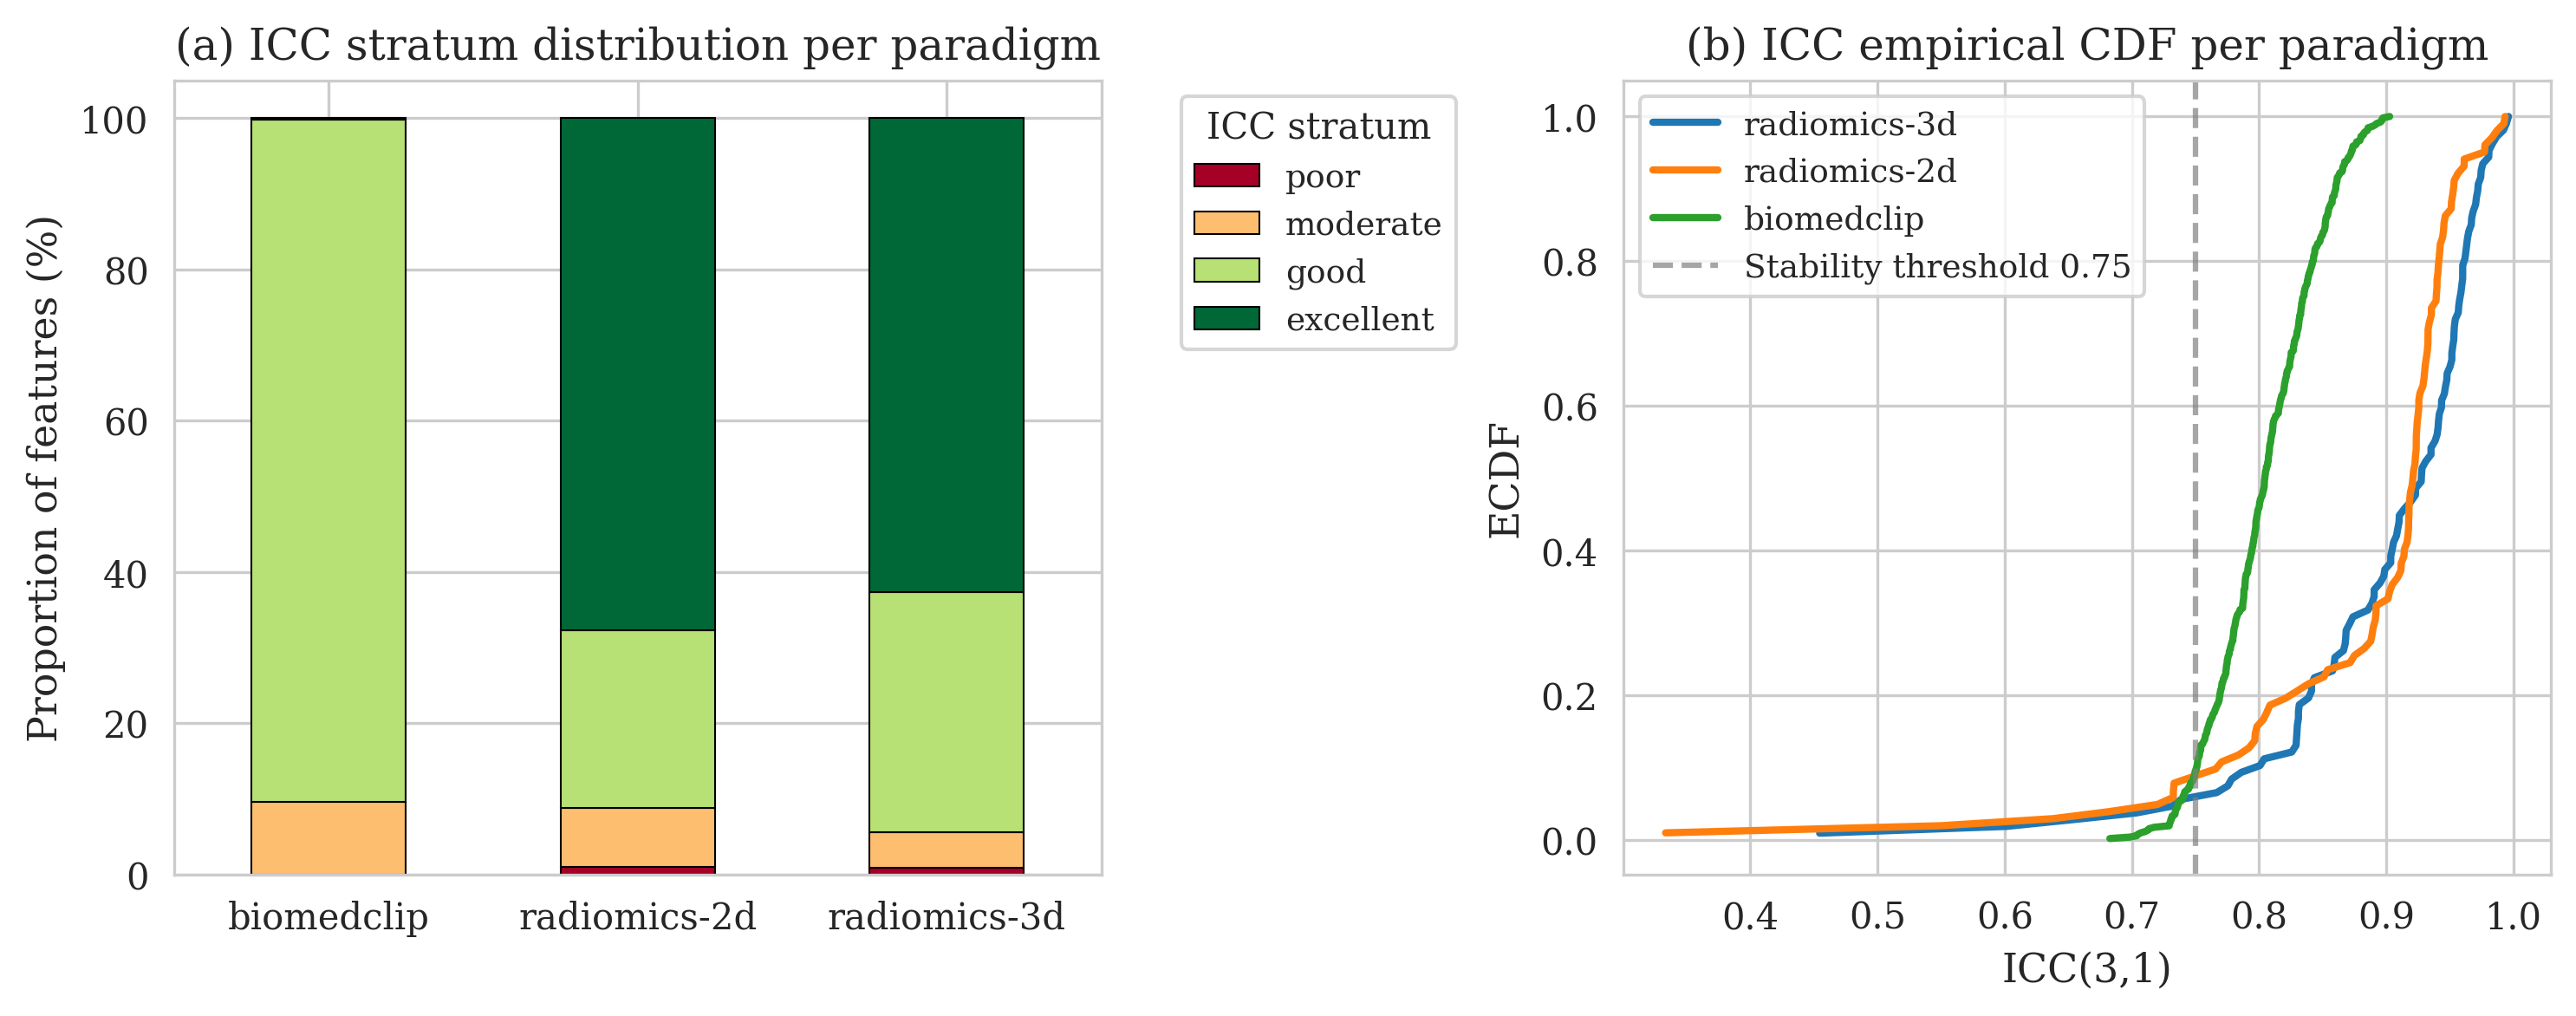
\includegraphics[width=0.9\textwidth]{figures/fig2_icc_distributions.png}
\caption{\textbf{ICC(2,1) distribution by paradigm.} (a)~Stacked-bar chart of ICC stratum proportions per paradigm. (b)~Empirical cumulative distribution functions of ICC per paradigm with the 0.75 stability threshold marked. The two PyRadiomics arms (3D, 2D) exhibit a bimodal pattern with a large excellent-stratum mode; BiomedCLIP exhibits a unimodal pattern concentrated in the good stratum with no poor-stratum dimensions.}
\label{fig:icc_dist}
\end{figure}

\subsection{Downstream classification and the effect of stability filtering (H2, H3)}

Out-of-fold 5-fold stratified cross-validated L2-logistic-regression classifiers~\cite{hosmer2013} achieved AUC values of 0.948 (95\% bootstrap CI 0.920--0.972) for PyRadiomics-3D, 0.955 (0.929--0.976) for PyRadiomics-2D, and 0.898 (0.861--0.931) for BiomedCLIP using the full unfiltered feature set per paradigm (Figure~3 and Table~2). Two unexpected findings arose from the pre-versus-post ICC-filter analyses. \textbf{Hypothesis H2 --- that FM embeddings would exhibit smaller AUC degradation than radiomics under stability filtering --- was rejected,} because both paradigms showed essentially zero AUC change under standard filtering (PyRadiomics-2D $\Delta$AUC = $+0.003$ at icc $\geq 0.75$; BiomedCLIP $\Delta$AUC = $-0.002$). \textbf{Hypothesis H3 --- that post-filter AUC would be non-inferior to pre-filter AUC at margin 0.020 --- was strongly supported for both paradigms.} PyRadiomics-2D AUC remained within $\pm 0.003$ of unfiltered at every filter threshold; BiomedCLIP AUC increased by $+0.014$ at the stricter ICC $\geq 0.85$ threshold despite an 84\% reduction in the active feature set ($512 \rightarrow 84$ dimensions). This result generalises the finding of Cosma~\textit{et al.}~2025~\cite{cosma2025} --- that ICC-based filtering can be unnecessary in modern radiomic pipelines --- to lung-CT data and to foundation-model embeddings.

The calibration metrics revealed an additional unanticipated finding. BiomedCLIP's unfiltered predictions were poorly calibrated (Brier score 0.144, expected calibration error 0.129), substantially worse than either PyRadiomics arm (Brier 0.074--0.077, ECE 0.030--0.057). Filtering BiomedCLIP to dimensions with ICC $\geq 0.85$ reduced the Brier score by 20\% ($0.144 \rightarrow 0.115$) and the expected calibration error by 50\% ($0.129 \rightarrow 0.065$), with simultaneous improvement in discrimination (AUC $0.898 \rightarrow 0.912$). This calibration-improvement effect was specific to BiomedCLIP and is consistent with an interpretation in which the moderately-stable BiomedCLIP dimensions encode perturbation-driven noise that adds uncertainty to the probability output without contributing malignancy signal.

\begin{figure}[H]
\centering

\includegraphics[width=0.85\textwidth]{figures/fig3_auc_forest.png}
\caption{\textbf{Out-of-fold AUC by paradigm and ICC filter threshold.} Forest plot with stratified-bootstrap 95\% confidence intervals over pooled out-of-fold predictions. The BiomedCLIP icc $\geq 0.90$ row is omitted because only one BiomedCLIP dimension crosses 0.90; the result would be a single-feature classifier rather than a meaningful filter.}
\label{fig:auc_forest}
\end{figure}

\subsection{Size-stratified subgroup analysis}

The structural correlation between nodule diameter and malignancy in LIDC (94\% of 6--10~mm nodules benign, 97\% of $>20$~mm nodules malignant) motivated the pre-specified diameter-stratified subgroup analysis. Within the 6--10~mm stratum ($n = 134$; 6\% malignant), all three paradigms achieved statistically indistinguishable AUC values: 0.762 (95\% CI 0.535--0.917) for PyRadiomics-3D, 0.774 (0.638--0.896) for PyRadiomics-2D, and 0.758 (0.611--0.899) for BiomedCLIP (Figure~4, left panel). Within the 10--20~mm stratum ($n = 99$; 74\% malignant), PyRadiomics-3D maintained a 0.095 AUC lead over BiomedCLIP (0.889 versus 0.794), although the confidence intervals overlapped (PyRadiomics-3D 0.805--0.960 versus BiomedCLIP 0.697--0.884) and the difference was not formally significant at this sample size (Figure~4, middle panel). The $>20$~mm stratum was not evaluable because the LIDC corpus contained only three benign nodules in this size range --- a structural consequence of Lung-RADS' clinical convention of treating $>20$~mm solid nodules as suspicious by definition~\cite{macmahon2017} (Figure~4, right panel).

\textbf{The aggregate AUC ranking (PyRadiomics 0.95 versus BiomedCLIP 0.90) is therefore substantially attributable to a size-malignancy confound in the cohort, rather than to a paradigm-level feature-quality difference.} Within the matched-size 6--10~mm stratum, the three paradigms converge to within $\sim 0.02$ AUC of each other. Within the 10--20~mm stratum, PyRadiomics-3D retains a modest advantage that is consistent with --- but not proof of --- a genuine paradigm-level feature-quality difference in mid-size nodules. The methodological implications for future foundation-model-versus-radiomics benchmarking studies are addressed in \S\,4.4.

\begin{figure}[H]
\centering
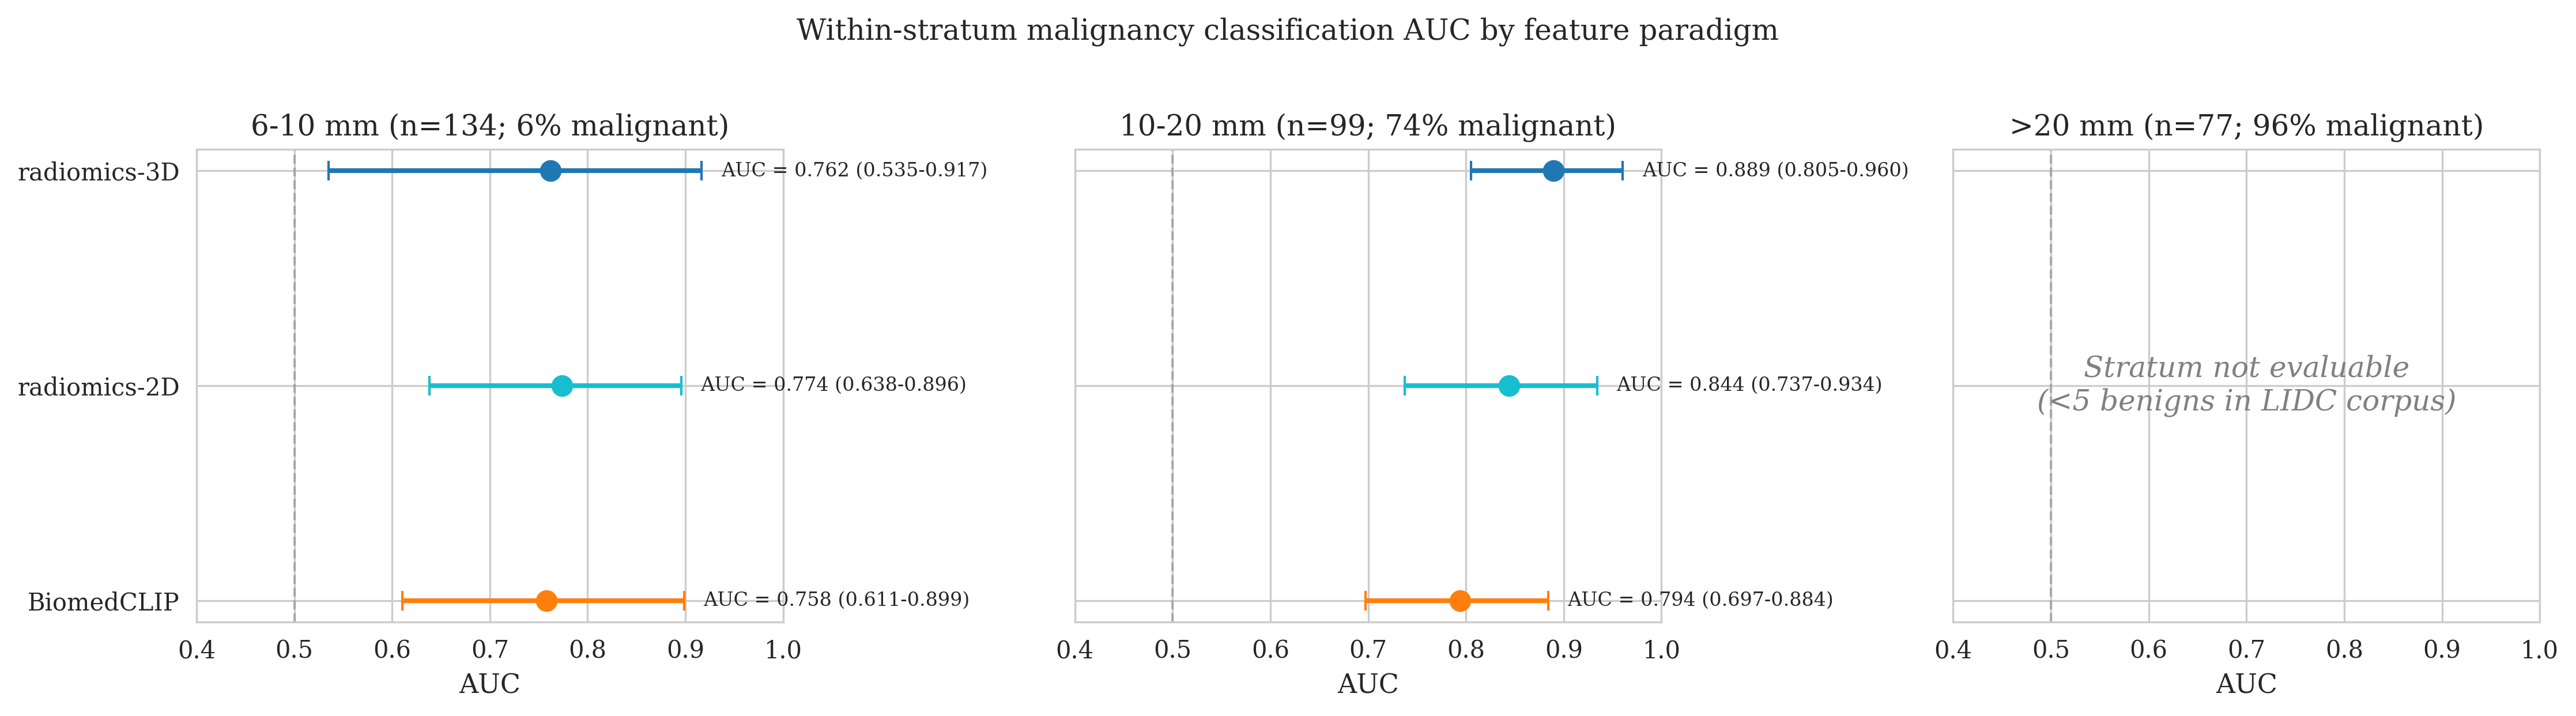
\includegraphics[width=\textwidth]{figures/fig4_stratified_auc.png}
\caption{\textbf{Diameter-stratified malignancy classification AUC by paradigm.} Three-panel forest plot showing within-stratum AUC values with bootstrap 95\% confidence intervals for the unfiltered feature set of each paradigm. The $>20$~mm stratum is not evaluable due to LIDC's structural scarcity of large benign nodules (3 of 76--77 total).}
\label{fig:stratified}
\end{figure}
